\section{Bāzes prototipa analīze}
Šajā darbā izstrādātā mikrokontroliera kodols par paraugu izmanto
D.~Perija (\termEn{D.~Perry}) ,,VHDL: Programming by Example'' grāmatā
piedāvāto procesora imple\-men\-tā\-ciju \cite{Perry-VHDL}.

Sākotnēji (rev.~01) izstrādātais kodols izmantoja gandrīz identisku
arhitektūru (bet atšķirīgu instrukciju kopu), bet
jau agri izstrādes procesā tika identificētas vairāki arhitektūras trūkumi,
no kuriem daži padarīja prototipu nesintezējamu.
Šī nodaļa apskata šos trūkumus un piedāvātos risinājumus.
Problēmu risinājumi šajā nodaļā apskatīti visai virspusēji,
to implementācijas detaļas, pēc iestrādes kodolā,
sīkāk apskatītas \ref{sec:cpu}~un \ref{sec:uC}~nodaļā.

\begin{figure}[thb]
	\centering
	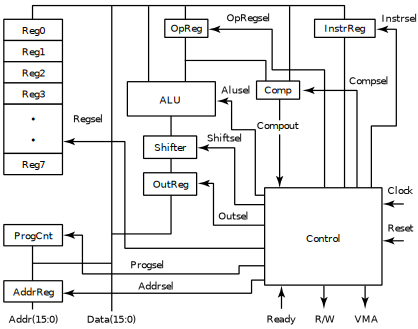
\includegraphics[scale=1.1]{perry-cpu}
	\caption[Bāzes prototipa uzbūves bloku diagramma.]
	        {Bāzes prototipa uzbūves bloku diagramma \cite[290.~lpp.]{Perry-VHDL}.}
	\label{fig:perry-cpu}
\end{figure}

D.~Perija procesors (turpmāk tekstā ,,bāzes prototips'')
ir vienkāršs 16 bitu procesors ar klasisku trīsstāvokļu 
centrālo datu šinu \cite{Flynn-arch}\cite{Heath}, un ar visām pamata
komponentēm (sk.~\ref{fig:perry-cpu}~att.), kas nodrošina bāzes prototipa
spēju izpildīt instrukcijas no tā instrukciju kopas.

\subsection{Iekšējā datu šina}
	Bāzes prototipa arhitektūra paredz kopēju, trīsstāvokļu iekšējo datu šinu
	(sk.~\ref{fig:perry-cpu}~att.).
	Šāda šinas uzbūve ir elektriski vienkārša, un ir shematiski viegli uztverama
	(sk.~\ref{fig:multidrop}~att.). Bet šāda uzbūve pieprasa šinas 
	,,arbitēšanu'', t.i.,~nepieciešams
	nodrošināt, ka tikai viena no šinai pievienotajām ierīcēm ir aktīvs devējs,
	kamēr pārējo ierīči izvadiem jābūt augstas impedances režīmā, kā arī
	jānodrošina lai pareizā ierīce (vai ierīces) šos datus nolasītu no šinas.

	\begin{figure}[thb]
		\centering
		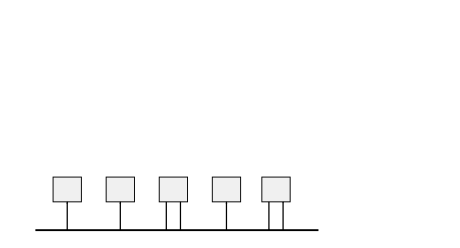
\includegraphics[scale=1.25]{multidrop}
		\caption{Kopējas trīstāvokļu datu šinas shēma.}
		\label{fig:multidrop}
	\end{figure}

	Galvenā problēma šādas šinas izmantošanai sintezējama kodola izstrādai ir
	fakts, ka vairums (vai pat visas) FPGA neatbalsta trīsstāvokļu
	loģiku, ko var secināt no fakta, ka neviena no apskatītajām FPGA neatbalsta
	loģisko bloku konfigurāciju ar atvērtā kolektora izejām
	\cite[18.~lpp.]{FusionFAQ}\cite{SmartFusionFabric}\cite{Xilinx7}.
	Tas nozīmē, ka pat ja sintēzes rīks atbalsta šādas šinas HDL aprakstu, tas
	ģenerēs ievērojami sarežģītāku struktūru, kas ,,emulē'' trīsstāvokļu datu šinu.

	Alternatīvas šinas uzbūvē ir ķēdes savienojumi vai maršrutējams tīkls.
	Maršrutējami tīklveida ir sarežģītas uzbūves, un pieprasa tikpat sarežģītu
	kontroles loģiku. Savukārt, ķēdes savienojumi ir pietiekami vienkārši,
	tādēļ tiek izvēlēti par risinājumu.

	\begin{figure}[thb]
		\centering
		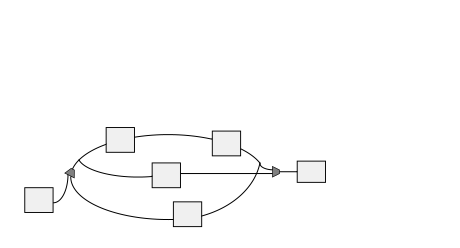
\includegraphics[scale=1.25]{chain}
		\caption{Vienvirziena cirkulāra ķēde ar atzarojumiem.}
		\label{fig:chain}
	\end{figure}

	Visai komplicēta ķēdes savienojumu struktūra ir redzama \ref{fig:chain}~attēlā,
	bet kas idejiski atbilst risinājuma rezultātam. 
	Ar ķēdes savienojumiem datu pārraide notiek vienā virzienā,
	tādējādi nav nepieciešamas bidirekcionālās pieslēgvietas, bet ir nepieciešamas
	atsevišķas pieslēgvietas datu ievadei un izvadei. Noslēdzot sazarojumus ar
	multipleksoriem arī zūd nepieciešamība pēc trīsstāvokļu loģikas.

	Ķēdes savienojumu priekšrocība ir arbitēšanas vienkāršums. Ierīces uz šinas
	jau ir savienotas ar datu saņēmejierīcēm, tādējādi vienīgā arbitēšana ir
	nodrošināt datu plūsmu (signalizēt datu nolasi) un sazarojumu noslēdzošo
	multipleksoru komutēšana.
	
	Ķēdes savienojumu šinas ieguvums ir arī tā potenciālais datu caurlaides
	apjoms (\termEn{troughput}), kas ir ievērojami lielāks, jo ierīces nav
	savienotas pie viena mezgla, kas kopējā datu šinā ir sastrēguma punkts
	(\termEn{bottleneck}). Datus dažādos ķēdes posmos var pārraidīt
	paralēli un šinas atzaru datu pārraides ātrums drīkst savā starpā 
	atšķirties.

	Tā kā procesora komponentēm nav nepieciešams komunicēt katrai ar katru, ir
	iespējams izveidot optimizētu kēžveida datu šinu, kur tieši savienotas ir tikai
	komponentes starp kurām notiek tieša komunikācija. Kodolā iestrādāto
	risināju skatīt \ref{sec:databus}~nodaļā.

\pagebreak[3]
\subsection{Instrukciju kopa}
	Bāzes prototips paredz vienkāršu instrukciju kopu, ar konstanta garuma
	5 bitu operāciju kodiem. Instrukciju kopa ir tipiska \termEn{Load/Store}
	principa procesoru arhitektūrām. \termEn{Load/Store} princips nosaka, ka
	visas aritmētiskās, loģiskās, bīdes un komparācijas darbības notiek
	ar vispārējā pielietojuma reģistru masīva reģistriem un datu apmaiņa ar
	operatīvo atmiņu notiek ar atmiņas nolases un ierakstes instrukcijām
	\cite[11.~lpp.]{Flynn-arch}	(sk.~\ref{sec:regArray}~nod.).
	Instrukcijas sadalāmas šādās grupās \cite[291.~lpp.]{Perry-VHDL}:
	\begin{itemize}
		\item \textbf{atmiņas nolases} (\termEn{load}) un \textbf{ierakstes}
			(\termEn{store}) instrukcijas, kuras
			veic datu apmaiņu starp reģistriem un operatīvo atmiņu;
		\item \textbf{zarošanās} instrukcijas, kas izmaina
			izpilāmā mašīnkoda (programmas) aktīvo pozīciju, un iekļauj
			nosacījuma un beznosacījuma zarošanās;
		\item instrukcijas, kuras veic \textbf{aritmētiskās} un 
			\textbf{bitu loģiskās} darbības ar reģistriem (operandiem);
		\item instrukcijas, kuras veic \textbf{bitu bīdes} reģistra
			(operanda) datiem.
	\end{itemize}
	
	Autorprāt, izmantotā instrukciju kopas izvēle ir racionāla, bet
	implementācija ir neoptimizēta. Pirmkārt, 5 bitu operācijas kods
	neefektīvi izmanto pieejamo 16 bitu mašīnvārdu
	(sk.~\ref{fig:5bit-opcode}~att.), un efektīvāk būtu izmantot mainīga
	garuma operācijas kodu.
	\begin{figure}[thb]
		\centering
		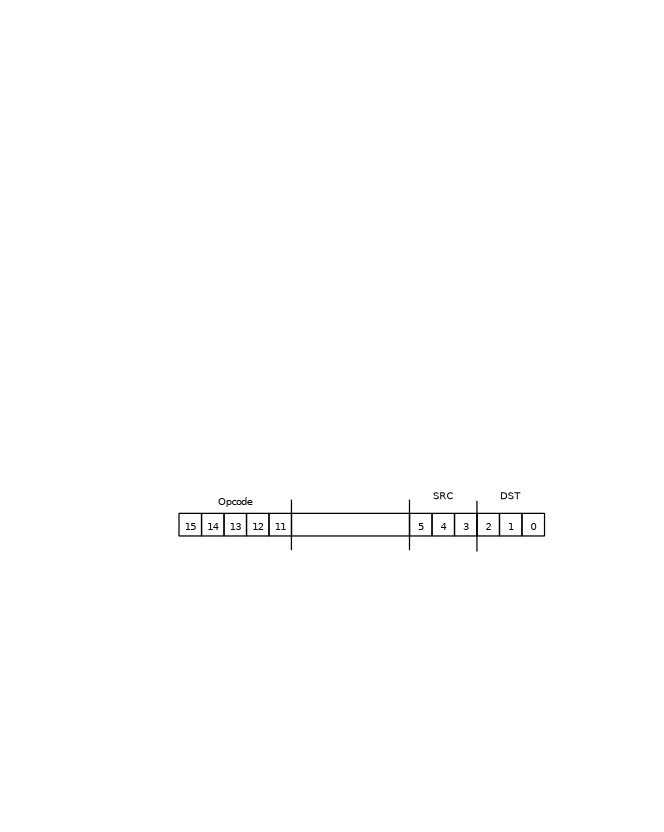
\includegraphics[scale=1.25]{perry-instr}
		\caption[5 bitu operācijas koda instrukcijas vārds.]
		        {5 bitu operācijas koda instrukcijas vārds \cite[292.~lpp.]{Perry-VHDL}.}
		\label{fig:5bit-opcode}
	\end{figure}
	
	Otrkārt, bāzes prototipa instrukciju operāciju kodi nes tikai kontroles
	iekārtai nozīmīgu informāciju un tiek pilnībā dekodēti dekodēšanas solī.
	Tas nozīmē, ka katrai instrukcijai nepieciešami savi, unikāli stāvokļi
	kontroles iekārtā (kas realizēta kā stāvokļu mašīna). Tā kā piem., 
	aritmētiskās instrukcijas (\texttt{ADD}, \texttt{SUB}, utt.)
	tiek izpildītas praktiski vienādi, iespējams veikt daļēju operācijas
	koda dekodēšanu un deleģējot atlikušā operācijas koda ,,dekodēšanu''
	ALU (sk.~\ref{sec:alu}~nod.), nododot tai nozīmīgu informāciju no
	operācijas koda. Tādējādi tiek panākti viekāršāka dekodēšanas loģika un 
	mazāk stāvokļu kontroles iekārtā, jo pietiek ar vienu šablonveida
	izpildes stāvokļu ķēdi.
	
	Kodola realizācijai, autors ir pilnībā no jauna izveidojis instrukciju
	kopu, kas iekļauj visas iepriekš minētās instrukciju grupas, bet
	konkrētās instrukcijas un to izpildes implementācija, kas izmanto minētās optimizācijas,
	ievērojami atšķiras (sk.~\ref{sec:instrSet}~nod.).
	
	Izstrādājot kodolu arī veikta papildus, arhitektūras specifiska
	optimizācija. Gan bāzes prototipa (sk.~\ref{fig:perry-cpu}~att.),
	gan izstrādātā kodola (sk.~\ref{fig:cpu-rev3}~att.) uzbūvē ALU un
	,,bitu bīdes iekārta'' atrodas uz viena signālceļa, kas nozīmē, ka
	izpildot gan bīdes, gan aritmētiskās instrukcijas dati tiek pārvadīti
	caur abām ierīcēm. Šo arhitektūras īpašību var izmantot izveidojot
	instrukciju, kas var veikt abas operācijas vienlaicīgi.
	Šādi kodolā implementēta \mnem{AR} instrukcija (sk.~\ref{sec:AR}~nod.).
	Tas arī nozīmē, ka visas aritmētiskās un bīdes instrukcijas ir izsakāmas
	ar šo ,,šabloninstrukciju'' vēl vairāk vienkāršojot kontroles iekārtas
	dekodēšanas loģiku un instrukciju izpildes stāvokļus.
	
\subsection{Komparators} \label{sec:perry-comp}
	Bāzes prototipā izmantotais komparators (sk.~\ref{fig:perry-comp}~att.),
	kura uzdevums ir salīdzināt	divus operandus (|a| un |b|), izvada
	rezultātu (|compout|) atkarībā pēc salīdzināšanas režīma signāla uz |sel|
	\cite[309.~lpp.]{Perry-VHDL}.
	\begin{figure}[thb]
		\centering
		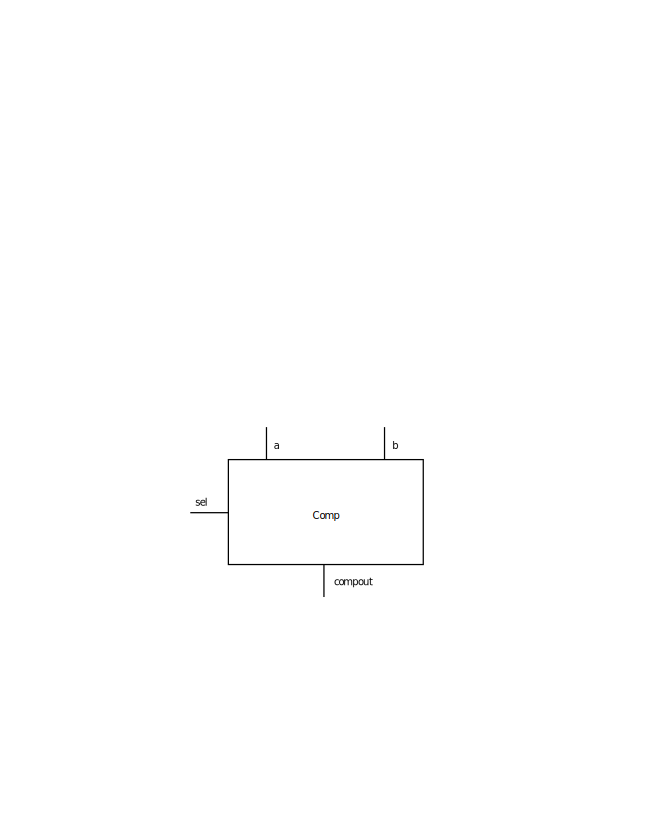
\includegraphics[scale=0.9]{perry-comp}
		\caption[Bāzes prototipa komparators.]
		        {Bāzes prototipa komparators \cite[309.~lpp.]{Perry-VHDL}.}
		\label{fig:perry-comp}
	\end{figure}
	
	Tiek definēti seši salīdzināšanas režīmi:
	\begin{itemize}
		\item operandu vienādība (|EQ|), kur |compout| ir |1|, ja |a|$=$|b|;
		\item operandu nevienādība (|NEQ|), kur |compout| ir |1|, ja |a|$\neq$|b|;
		\item operands |a| stingri lielāks (|GT|), kur |compout| ir |1|, ja |a|$>$|b|;
		\item operands |a| nestingri lielāks (|GTE|), kur |compout| ir |1|, ja |a|$\geq$|b|;
		\item operands |a| stingri mazāks (|LT|), kur |compout| ir |1|, ja |a|$<$|b|;
		\item operands |a| nestingri mazāks (|LTE|), kur |compout| ir |1|, ja |a|$\leq$|b|.
	\end{itemize}
	
	Šiem režīmiem eksistē ,,pretsakarības'', piem.~|EQ| ir pretējs |NEQ| un
	|GT| pretējs |LTE|, kas nozīmē ka šie režīmi ir redundanti. Izslēdzot
	redundantos režīmus iegūstam trīs: |LT|; |EQ|; |GT|, kas arī apzīmē
	trīs iespējamos operandu savstarpējos stāvokļus.
	Sekojot no matemātiskās aksiomas var pierādīt, ka
	\[
		\neg (a>b) \land (a \neq b) \iff (a<b)
	\]
	skaidri parādot, ka pārbaudot jebkurus divus stāvokļus trešais
	nosakāms pēc noklusējuma.
	\pagebreak[3]
	
	Tad tā vietā lai nodotu vienu no sešiem pārbaudes režīmiem,
	varam optimizēt, likvidējot režīmu pārslēgšanu vispār, un vienmēr izvadot
	rezultātu no divu operandu savstarpējo stāvokļu pārbaudes.
	
	Kodola realizācijā izmantots ,,bezrežīmu'' komparators, kas 
	divus signāla bitus, kas attiecīgi norāda 
	vai operands |a| ir vienāds ar |b|, 
	un vai operands |a| ir lielāks par |b| (sk.~\ref{sec:comp}~nod.).
	Protams šāda implementācija nozīmē papildus loģiku kontroles iekārtā,
	bet tās implementācija ir visai vienkārša, kā apskatīts
	\ref{sec:branching}~nodaļā.

%\subsection{Kontroles iekārta}
%	\todo
